\documentclass{beamer}
\usepackage[english,russian]{babel}
\usepackage[utf8]{inputenc}

\usepackage{xskak}
\usepackage{chessboard}

\usepackage{amsmath,amssymb,cite,graphicx}
\usepackage{subfigure}
\usepackage{url}

% Стиль презентации
\usetheme{Frankfurt}
\begin{document}
\title{Математическое моделирование\\ когнитивных процессов при игре в шахматы} 
\author{Афанасьева Анастасия}
%\institute{Московский государственный университет имени М.",В.",Ломоносова}
\institute{Московский государственный университет имени М.",В.",Ломоносова\\
    \vspace{0.7cm}
    Научный руководитель:  Афонин Сергей Александрович \\
    \vspace{0.7cm}
}
\date{Москва, 2016} 
% Создание заглавной страницы
\frame{\titlepage} 

% Автоматическая генерация содержания
\frame{\frametitle{Содержание}\tableofcontents}



\section[Зачем]{Зачем этим нужно заниматься?}
%\section[Обзор]{Обзор существующих подходов}
\subsection{Как думает человек}
%\subsection{Как думает человек}
\begin{frame}{Психология принятия решений} 
Игра в шахматы является традиционным предметом изучения психологии принятия решений. Первые работы опубликованы в 1894 году. 

\bigskip
Большой вклад внёсли работы А. де Гроота (1946), Саймона (1982) и другие. Проводились исследования по двум основным направлениям:
\begin{itemize}
\item Восприятие (запоминание позиции)
\item Принятие решения при выборе хода
\end{itemize} 
\end{frame}

\begin{frame}{Восприятие}
\textbf{Эксперимент} 
\begin{itemize}
\item На время $t_1 = 5$с предъявлялась позиция. Через время $t_2 = 30$с предлагалось её восстановить. Анализровался порядок и число правильно восстановленных фигур. 
\end{itemize}
\textbf{Результаты}
\begin{enumerate}
\item На реальных позициях есть различие между экспертами и новичками.
\item Для случайных позиций различия нет.
\item Фигуры рассматриваются логически связанными группами.
\item Некоторые позиции восстанавливаются по ассоциации с другими партиями.
\end{enumerate}
\end{frame}


\begin{frame}{Принятие решения}
\textbf{Эксперимент}
\begin{itemize}
\item Экспертам предъявлялась позиция из реальной партии. Предлагалось выбрать наилучший ход. Производить рассуждения требовалось вслух.   
\end{itemize}
\textbf{Результаты}
\begin{enumerate}
\item Рассматривается небольшое число ходов-кандидатов.
\item Небольшая глубина анализа (до 5 ходов) вне зависимости от мастерства.
\item Дерево анализа содержит $20-80$ узлов. 
\item Частые возвращения назад: анализ хода или эпизода часто повторяется.  
\end{enumerate}
\end{frame}

\begin{frame}{Теория прогрессивного углубления}
По результатам проведенных исследований де Гроотом были выделены основные фазы мышления шахматиста\footnotemark{}
\begin{itemize}
\item ориентировка (выделение группы ключевых фигур);
\item разведка (пробы нескольких ходов);
\item обработка (систематический глубокий просчёт вариантов);
\item доказательство (проверка надёжности результата).
\end{itemize}
\footnotetext{de Groot A.D., 1946, 2008. Thought and Choice in Chess,  Amsterdam University Press // Amsterdam Academic Archive.}
\end{frame}

\AtBeginSubsection[]
  {
     \begin{frame}<beamer>
     \frametitle{Содержание}
     \tableofcontents[currentsubsection]
     \end{frame}
  }

\subsection{Как играют современные программы}
%\subsection{Существующие подходы}

\begin{frame}{Полный перебор}
В 1913 году в работе Цермело\footnotemark{} было доказано существование оптимальной стратегии игры с полной информацией.
Подход состоит в построении полного дерева игры.
\begin{figure}
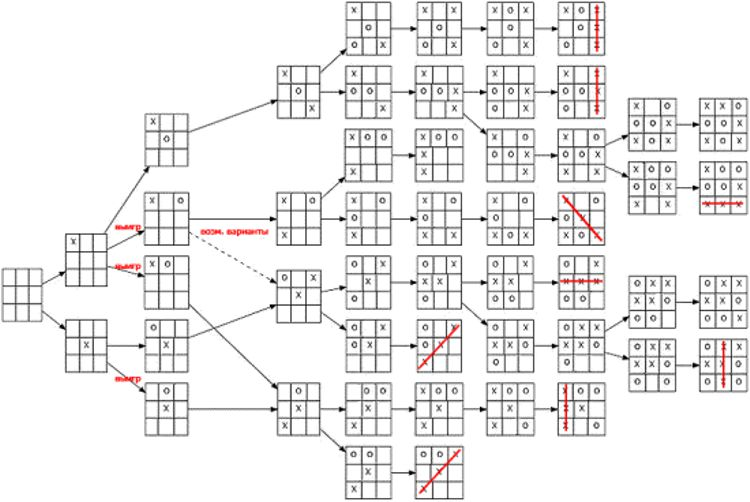
\includegraphics[scale=0.3]{./pictures/xoxo.jpg}
\end{figure}
\footnotetext{Е. Zermelо, Obereine Anwendung der Mengenlehre attfdie Theorie des Schachspiels (Cambridge, 1913)}
%Zermelo E. Über eine Anwendung der Mengenlehre auf die Theorie des Schachspiels //Proceedings of the fifth international congress of mathematicians. – II, Cambridge UP, Cambridge, 1913. – Т. 2. – С. 501-504.
\end{frame}

%\begin{frame}{Полное дерево игры}
%\begin{figure}
%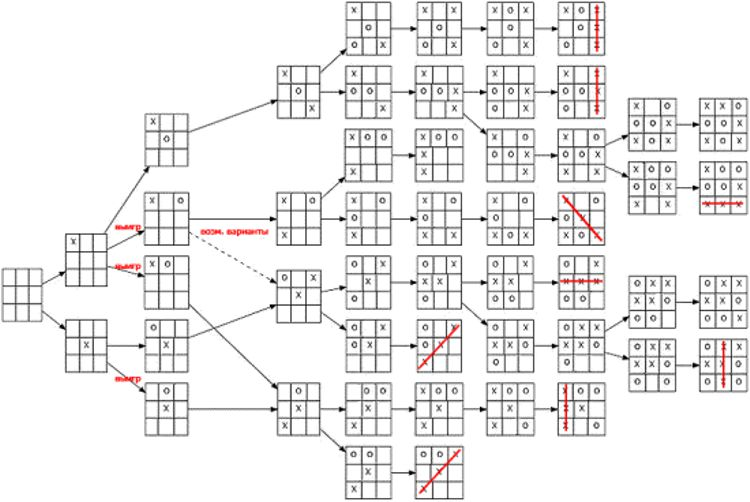
\includegraphics[scale=0.5]{./pictures/xoxo.jpg}
%\end{figure}
%\end{frame}

\begin{frame}{Особенности переборного подхода}
\begin{itemize}
\item После $m$ ходов дерево игры содержит порядка $d^m$ листов, где $d$ -- среднее количество возможных ходов в позиции.
\item Для крестиков-ноликов $d \approx 5$, для шахмат $d \approx 60$, для~го~$d \approx 400$. 
\item Построение требует большой вычислительной мощности.
\item Включает в себя множество очевидно бессмысленных ходов.
\item Проводится сокращение дерева с помощью различных эвристических методов (minimax, alpha-beta и другие).
\item У современных программ, с учетом отсечений, осуществляется перебор $100.000$ позиций в секунду. (<<Rybka>>)
\end{itemize}
\end{frame}

%ГУГЛ!
\begin{frame}{Нейронные сети}
Игровые задачи часто используются как способ тестирования и проверки эффективности применения алгоритмов автоматического обучения\footnotemark{}. 
\begin{itemize}
\item Лучший ход рассматривается как функция от текущего расположения фигур на доске.
\item Требует больших объемов обучающих данных.
\item Возможно самообучение.
\item Достигнуты выдающиеся результаты: 13-ти слойная нейронная сеть
  одержала победу 4:1 над одним из сильнейших игроков мира в го Ли
  Седолем.
\item Объяснить выбор конкретного хода нельзя.
\end{itemize}
\footnotetext{Silver D. et al. Mastering the game of Go with deep neural networks and tree search //Nature. – 2016. – Т. 529. – №. 7587. – С. 484-489.}
\end{frame}


%\subsection{Сравнение}

%\subsection{Сравнение}
\begin{frame}{И всё-таки зачем}
\begin{figure}
%Шахматные турниры...
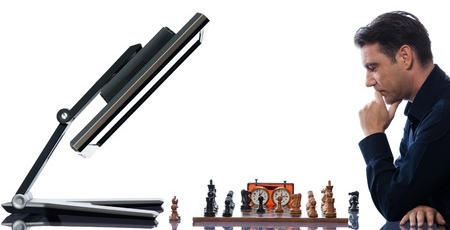
\includegraphics[scale=0.55]{./pictures/vs.png}
\end{figure}
\begin{columns}
\column{0.5\textwidth}
\begin{itemize}
\item Позиции анализируются независимо
\item Большой объем обрабатываемых данных
\item Сложно объяснить принципы выбора хода
\end{itemize}
\column{0.5\textwidth}
\begin{itemize}
\item Блочное восприятие
\item Ограниченный перебор
\item Прогрессивное углубление
\item Долгосрочное планирование
\end{itemize}
\end{columns}

\smallskip
Нет реализаций, учитывающих психологические аспекты.
\end{frame}

\endinput

\begin{frame}{Зачем этим нужно заниматься?} 
\begin{itemize}
\item Шахматы, как игра с полной информацией, сводится к решению задачи комбинаторной оптимизации.
\item Человек способен эффективно решать подобные задачи неформальным способом.
\item Существующие игровые программы основываются на иных методах решения.
\item В точности определить подход, используемый человеком, на данный момент не удалось.
\end{itemize}
\end{frame}


\begin{frame}{Сравнение и почему ничего не подходит}
\begin{itemize}
\item  практические результаты достигнутые программами значительно превосходят человеческие. Обыграли человека во всех играх (в т.ч. Го)
\item Анализ большого количества данных (статистических или в ходе построения дерева)
\item Не учитываются психологические аспекты.
\item Отсутствует стратегическое дальносрочное планирование.
\item Процесс мышления человека смоделировать не удалось.
\end{itemize}
\end{frame} 


\AtBeginSection[]
  {
     \begin{frame}<beamer>
     \frametitle{Содержание}
     \tableofcontents[currentsection]
     \end{frame}
  }
  
\section{Метод М.М. Ботвинника}
%\subsection{Подход М.М.Ботвинника}
\begin{frame}{Подход М.М.Ботвинника}
Ботвинник предлагал анализировать расположение фигур на статической доске. Для этого необходимо: 
\begin{itemize}
\item определить локальные цели для данной позиции;
\item наметить план достижения цели;
\item проверить осуществимость плана;
\item объединить планы в единое представлене о позиции;
\item определить оптимальную последовательность действий.
\end{itemize}
Данный подход рассматривался, как средство решения широкого класса комбинаторно-оптимизационных задач.
\end{frame}

\subsection{Основные понятия}
\begin{frame}{Основные понятия}
\begin{description}
\item[Траектория] последовательность полей движения фигуры на пустой доске
\item[Горизонт] максимальная длина рассматриваемых траекторий
\item[Цель] фигуры противника или поля
\item[Подцепочка] действия, направленные на достижение цели
\item[Цепочка] совокупность действий, направленных на достижение цели
\item[Вилочность] совпадение частей цепочек
\item[Оценка фигуры] числовая характеристика <<полезности>> фигуры
\item[Время успевания] допустимое число ходов для защиты от атаки противника
\end{description}
\end{frame}

\begin{frame}{Основные понятия: пример цепочки}
\begin{columns}
\column{0.5\textwidth}
\begin{figure}[t]
  \centering
  \subfigure[1.]{%
    \scalebox{0.8}{%
      \setchessboard{showmover=true}%
      \chessboard[setpieces={Pa5, Na7, bh3},%
      arrow=stealth,%
      linewidth=.25ex,%
      padding=1ex,%
      color=red!55!white,%
      pgfstyle=straightmove,%
      shortenstart=1ex,%
      showmover=false,%
      markmoves={a5-a8},%
      padding=10ex,%
      shortenend=1ex%
      %, markmoves={f3-g3,g3-h4}%
      ]%
    }%
  }
\end{figure}
\column{0.5\textwidth}
\textbf{Цель} - достижение пешкой поля a8 \\
\textbf{Траектория} - a5-a6-a7-a8. \\
\pause
\textbf{Подцепочка-1} - освобождение траектории a7-b5, a7-c6, a7-c8. \\
\pause
\textbf{Подцепочка-1} - защита противника h3-g2-(a8), h3-f1-(a6) \\
\pause
\textbf{Подцепочка-2} - поддержка a7-b5-c7-(a8, a6), a7-c8-b6-(a8)
\end{columns}
\end{frame}


\subsection{Примеры и обобщения}
\begin{frame}{Примеры на модельных задачах} %без королей
Позиция, \\
анализ, \\ 
пример цепи (цель). 
\end{frame}

\begin{frame}{Обобщение}
Лингвистическая геометрия \\
Экономика
\end{frame}

\begin{frame}{Проблемы} % +диаграммы на каждый пункт с примерами 
Динамический горизонт событий \\
Динамическая оценка фигур и цепей \\
Связь между цепочками \\
Траектории с подвижной целью \\
Оптимальность цепи
%НЕТ ФОРМАЛИЗАЦИИ!! \\
\end{frame}


%здесь начинается своё
\section{Своё}
%%\subsection{Подход М.М.Ботвинника}
\begin{frame}{Подход М.М.Ботвинника}
Ботвинник предлагал анализировать расположение фигур на статической доске. Для этого необходимо: 
\begin{itemize}
\item определить локальные цели для данной позиции;
\item наметить план достижения цели;
\item проверить осуществимость плана;
\item объединить планы в единое представлене о позиции;
\item определить оптимальную последовательность действий.
\end{itemize}
Данный подход рассматривался, как средство решения широкого класса комбинаторно-оптимизационных задач.
\end{frame}

\subsection{Основные понятия}
\begin{frame}{Основные понятия}
\begin{description}
\item[Траектория] последовательность полей движения фигуры на пустой доске
\item[Горизонт] максимальная длина рассматриваемых траекторий
\item[Цель] фигуры противника или поля
\item[Подцепочка] действия, направленные на достижение цели
\item[Цепочка] совокупность действий, направленных на достижение цели
\item[Вилочность] совпадение частей цепочек
\item[Оценка фигуры] числовая характеристика <<полезности>> фигуры
\item[Время успевания] допустимое число ходов для защиты от атаки противника
\end{description}
\end{frame}

\begin{frame}{Основные понятия: пример цепочки}
\begin{columns}
\column{0.5\textwidth}
\begin{figure}[t]
  \centering
  \subfigure[1.]{%
    \scalebox{0.8}{%
      \setchessboard{showmover=true}%
      \chessboard[setpieces={Pa5, Na7, bh3},%
      arrow=stealth,%
      linewidth=.25ex,%
      padding=1ex,%
      color=red!55!white,%
      pgfstyle=straightmove,%
      shortenstart=1ex,%
      showmover=false,%
      markmoves={a5-a8},%
      padding=10ex,%
      shortenend=1ex%
      %, markmoves={f3-g3,g3-h4}%
      ]%
    }%
  }
\end{figure}
\column{0.5\textwidth}
\textbf{Цель} - достижение пешкой поля a8 \\
\textbf{Траектория} - a5-a6-a7-a8. \\
\pause
\textbf{Подцепочка-1} - освобождение траектории a7-b5, a7-c6, a7-c8. \\
\pause
\textbf{Подцепочка-1} - защита противника h3-g2-(a8), h3-f1-(a6) \\
\pause
\textbf{Подцепочка-2} - поддержка a7-b5-c7-(a8, a6), a7-c8-b6-(a8)
\end{columns}
\end{frame}


\subsection{Примеры и обобщения}
\begin{frame}{Примеры на модельных задачах} %без королей
Позиция, \\
анализ, \\ 
пример цепи (цель). 
\end{frame}

\begin{frame}{Обобщение}
Лингвистическая геометрия \\
Экономика
\end{frame}

\begin{frame}{Проблемы} % +диаграммы на каждый пункт с примерами 
Динамический горизонт событий \\
Динамическая оценка фигур и цепей \\
Связь между цепочками \\
Траектории с подвижной целью \\
Оптимальность цепи
%НЕТ ФОРМАЛИЗАЦИИ!! \\
\end{frame}

\begin{frame}{...}

\end{frame}

\subsection{Формализация}
%\subsection{Технический аспект}
\begin{frame}{Технические шаги для решения задачи}
Для решения содержательных задач необходимо реализовать ряд вспомогательных функций:
\begin{itemize}
\item определить соответствие хода правилам;
\item строить траектории на пустой доске;
\item оценивать последовательность взятий и величину размена на поле;
\item находить фигуры, способные повлиять на размен, и позиции, которые им необходимо занять;
\end{itemize}
Все эти функции были реализованы.
%построение цепочки
\end{frame}

\begin{frame}{Пример цепочки: дерево (повтор)}
\begin{tabular}{ll}
\begin{tikzpicture}
\begin{scope}[every node/.style={circle,thick,draw}]
    \node (A5) at (0,0) {a5};
    \node (A6) at (2,0) {a6};
    \node (A7) at (4,0) {a7};
    \node (A8) at (6,0) {a8};
    \node (NA7) at (2,2) {a7};
    \node (B5) at (4,2) {b5};
    \node (C7) at (6,2) {c7};
    \node (H3) at (4,-2) {h3};
    \node (G2) at (6,-2) {g2};
\end{scope}

\begin{scope}[%>={Stealth[black]},
              every node/.style={fill=white,circle},
              every edge/.style={draw=red,very thick}]
    % подцепочка 0
    \path [->] (A5) edge (A6);
    \path [->] (A6) edge (A7);
    \path [->] (A7) edge (A8);
    % Защита
    \path [->] (H3) edge (G2);
    \path [->] (G2) edge[gray, draw=gray, dashed] (A8);
    % Отступление 
    \path [->] (NA7) edge (B5);
    \path [->] (B5) edge (C7);
    \path [->] (B5) edge[gray, draw=gray, dashed] (A7);
    \path [->] (C7) edge[gray, draw=gray, dashed, bend left] (G2);
    %\path [->] (B) edge[bend right=60] node {$1$} (E); 
\end{scope}
\end{tikzpicture}
&
{\scalebox{0.5}{\showDiagram{Pa5, Na7, bh3}{}}}
\end{tabular}

Пунктиром отмечены поля, к которым <<подтянуты>> соотвествующие подцепочки.
\end{frame}

\begin{frame}{Формальная модель}
Множество полей доски $\mathcal{S} \coloneqq \{a1, b1, \dots, h8\}$.\\
Типы полей $\mathcal{ST} \coloneqq \{stop, internal\}$ --- поля остановки или промежуточные.\\
Множество типов фигур $\mathcal{K} \coloneqq \{ K, Q, R, B, N, P \}$ \\
Цвета соперников $\mathcal{C} \coloneqq \{black, white\}$ \\
Траектория $\mathcal{T} \in \left( \mathcal{S} \times \mathcal{ST} \right)^+$ --- упорядоченный набор полей.\\
Доска $\Delta  \colon \mathcal{S} \to \mathcal{K} \times \mathcal{C} $ --- соответсвтие полю фигуры (типа и цвета). \\
Цепочка $Chain \coloneqq \langle color, traj, sa \rangle$,  где $color \in \mathcal{C}$ --  цвет цепочки, $traj \in \mathcal{T}$ -- основная траектория цепочки, $sa \subset \mathbb{N} \times 2^{\mathtt{Chains}}$ -- множество вспомогательных действий для проходимости поля траектории. \\
В этом контексте понятие фигуры принимает вид всех цепочек одного цвета с общим началом траекторий.
\end{frame}

%картинка фигуры =_=
\begin{frame}{Пример фигуры}
\begin{tabular}{ll}
\begin{tikzpicture}
\begin{scope}[every node/.style={circle,thick,draw}]
    \node (A7) at (0,0) {a7};
    \node (B5) at (2,0) {b5};
    \node (C7) at (4,0) {c7};
    \node (B6) at (4,-2) {b6};
    \node (B8) at (4,2) {b8};
    \node (A6) at (6,2) {a6};
    \node (A8) at (6,-2) {a8};
    \node (C6) at (2,2) {c6};
    \node (C8) at (2,-2) {c8};
\end{scope}

\begin{scope}[%>={Stealth[black]},
              every node/.style={fill=white,circle},
              every edge/.style={draw=red,very thick}]
    % подцепочка 0
    \path [->] (A7) edge (B5);
    \path [->] (B5) edge[red, draw=red, dashed] (C7);
    \path [->] (C7) edge[red, draw=red, dashed] (A6);
    \path [->] (C7) edge[red, draw=red, dashed] (A8);
    % Защита
    \path [->] (A7) edge[gray, draw=gray] (C6);
    \path [->] (C6) edge[gray, draw=gray, dashed] (B8);
    \path [->] (B8) edge[gray, draw=gray, dashed] (A6);
    \path [->] (A7) edge[gray, draw=gray] (C8);
    \path [->] (C8) edge[gray, draw=gray, dashed] (B6);
    \path [->] (B6) edge[gray, draw=gray, dashed] (A8);
    %\path [->] (B) edge[bend right=60] node {$1$} (E); 
\end{scope}
\end{tikzpicture}
&
{\scalebox{0.5}{\showDiagram{Pa5, Na7, bh3}{}}}
\end{tabular}

Пунктиром отмечены цепочки, <<поддерживающие>> размен.
\end{frame}

\endinput
\begin{frame}{Формализация: построение цепи}
\begin{columns}
\column{0.5\textwidth}
\begin{figure}
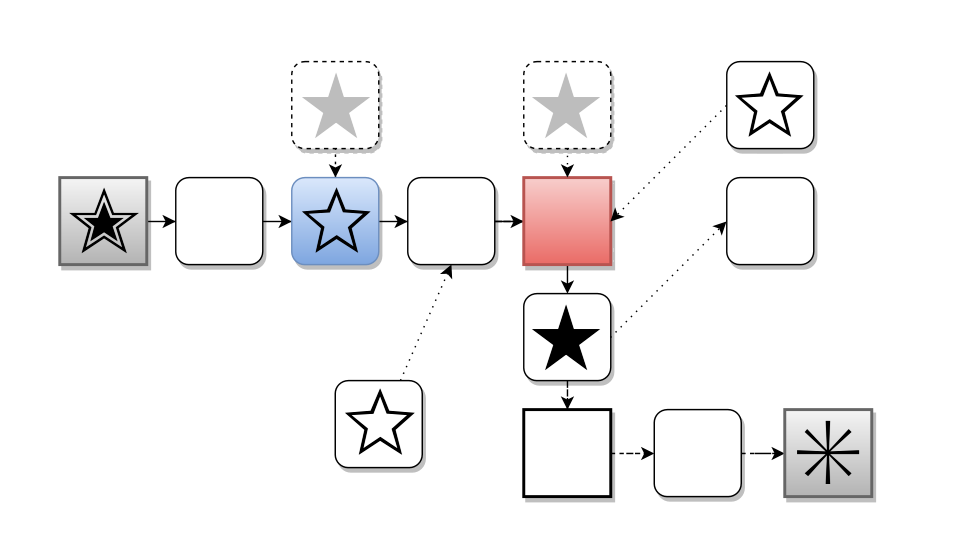
\includegraphics[scale=0.2]{./pictures/chain.png}
\end{figure}
\column{0.5\textwidth}
\begin{itemize}
\item определение цели для фигуры
\item построение траектории - подцепи-0
\item определение проходимости траектории
\item построение подцепей высших порядков
\end{itemize}
\end{columns}
Так как цепи весьма вариативны, необходимо выбрать оптимальное поддерево подцепей для цепи - произвести локальную оптимизацию.
\end{frame}

\begin{frame}{Формализация: оптимизация при построении}
\begin{columns}
\column{0.5\textwidth}
\begin{figure}
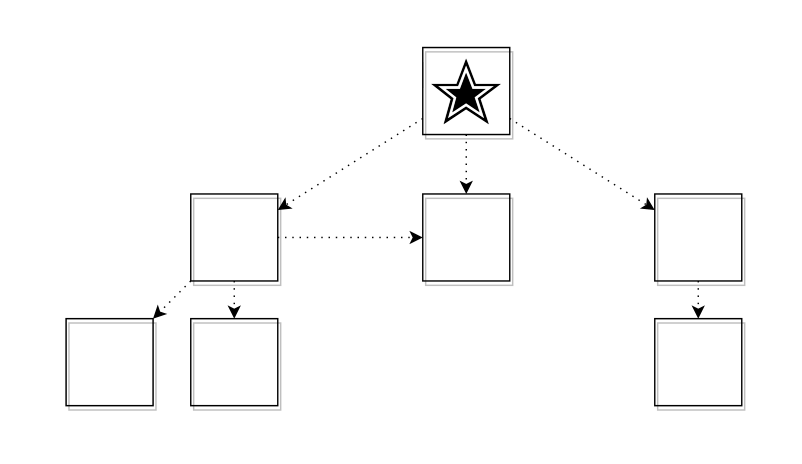
\includegraphics[scale=0.2]{./pictures/piece.png}
\end{figure}
\column{0.5\textwidth}
\begin{itemize}
\item квадраты - поля доски
\item с каждым полем связаны цепи
\item количество и качество цепей влияет на вес хода
\end{itemize}
\end{columns}
Глобальная оптимизация заключается в уточнении оценки для фигур по числу цепей, что может повлиять на уже построенные цепи
\end{frame}



\subsection{Результаты}
\begin{frame}{Оценочная функция}
Для вычисления оценочной функции цепочки необходимы: \\
$ep_{chain} \left(n\right) \in 2^{\mathtt{Pieces}}$ --- множество фигур, участвующих в размене на $n$-ом поле траектории. \\
$value\left(p\right) \in \mathbb{Z}$ --- стоимость фигуры, белые фигуры имеют положительную оценку, черные -- отрицательную.\\ 
$len_{chain}\left(traj\right) \in \mathbb{N}^+$ --- длина траектории. \\
Определим оценочную функцию $\varphi \colon \mathtt{Chains} \to \mathbb{N}$:
$$
 \varphi \left( ch \right) = \sum_{k \in \left[0, l\right]} \sum_{ p \in ep\left(k\right)} value\left(p\right) + \sum_{sch \in sa\left(k, traj\right)} \varphi\left(sch\right)
$$
Согласно полученной оценке, построим граф, узлами которого являются оцененные цепочки, имеющие одинаковую изначальную структуру - подцепочку-0.
\end{frame}

\begin{frame}{Граф цепочек}
 Если две цепочки $\left(\Gamma_{0, 0}, \alpha_0\right)$ и $\left(\Gamma_{0, 1}, \alpha_1\right)$ таковы, что $\alpha_0 > \alpha_1$, то проводится ребро черного цвета. Это означает, что черные могут улучшить оценку в свою пользу. 
%\begin{tabular}{ll}
\begin{tikzpicture}
\begin{scope}[every node/.style={circle,thick,draw}]
    \node (00) at (0,0) {$\Gamma_{0, 0}, \alpha_0$};
    \node (01) at (3,0) {$\Gamma_{0, 1}, \alpha_1$};
    \node (21) at (6,0) {$\Gamma_{2, 1}, \alpha_4$};
    \node (11) at (3,-3) {$\Gamma_{1, 1}, \alpha_2$};
    \node (10) at (0,-3) {$\Gamma_{1, 0}, \alpha_3$};
    \node (22) at (9,0) {$\Gamma_{2, 2}, \alpha_5$};
    \node (23) at (6,-3) {$\Gamma_{2, 3}, \alpha_6$};
    \node (24) at (9,-3) {$\Gamma_{2, 4}, \alpha_7$};
\end{scope}
\begin{scope}[%>={Stealth[black]},
              every node/.style={fill=white,circle},
              every edge/.style={draw=black,very thick}]
    % подцепочка 0
    \path [->] (00) edge (01);
    \path [->] (11) edge (10);
    \path [->] (21) edge (22);
    \path [->] (21) edge (23);
    \path [->] (21) edge (24);
    \path [->] (01) edge[dashed] (21);
    \path [->] (01) edge[dashed] (11);
    \path [->] (10) edge[dashed] (00);
\end{scope}
\end{tikzpicture}
%&\end{tabular}
\end{frame}

\begin{frame}{Оптимальная цепочка}
Выбор цепочки с нашей стороны определяется максимальным значением оценочной функции, в то время как противник, наоборот, стремится реализовать цепочку, которая её минимизирует. \\
То есть, противник выбирает цепочку той же структуры нашего цвета, заменяя в ней подцепочки своего цвета, чтобы максимально уменьшить оценку. \\
В случае цикла, \textbf{оптимальным} считается тот узел, в котором при наилучшем выборе противника, мы имеем возможность улучшить оценку. \\
При линейной структуре \textbf{оптимальна} листовая вершина с максимальной оценкой.
\end{frame}

\begin{frame}{Трудности нахождения оптимальной цепочки} %граф, содержащий всё.
Основная трудность заключается в построении графа цепочек, так как при построении необходимо включать в него всевозможные цепочки. \\
Вместо полного перебора вариантов, хотелось бы иметь структуру, достраивающую подцепи динамически, если возникает такая необходимость.\\
Так же оценка фигур не является фиксированным числом, а зависит от цепочек, в которых она участвует. \\
Одна и та же фигура в одной цепочке может выполнять несколько функций, то есть, участвовать в нескольких подцепочках. В зависимости от временных рамок, её поведение так же может различаться. 
%Непонятно об оценке фигур и связях между фигурами в цепочках (в двух подцепях по-разному, можно ли ходить вдоль траектории, или нельзя).
\end{frame}

\endinput
\begin{frame}{Результаты}
{{$$\begin{cases}
\alpha_0 < \alpha_1 \\
\alpha_1 > \alpha_2 \\
\alpha_2 < \alpha_3 \\
\alpha_3 > \alpha_0
\end{cases}
$$}}
На данный момент программная реализация: \\
\begin{itemize}
\item находит пути на пустой доске (подцепи-0); \\
\item маркирует поля траектории по признаку проходимости; \\
\item находит кандидатные подцепи. \\
\end{itemize}
\end{frame}


\section{Заключение}
%\subsection{Выводы}

\begin{frame}{Ближайшие цели}
\begin{itemize}
\item Построение одной вариативной цепочки \\
\item Локальная проверка гипотезы \\
\item Глобальная оптимизация - объединение цепей \\
\item Глобальная проверка гипотезы
\end{itemize}
\end{frame}

\begin{frame}{}

\begin{center}
{\Huge Спасибо за внимание}
\end{center}

\end{frame}

\end{document}